% Created 2017-08-20 Sun 19:22
% Intended LaTeX compiler: pdflatex
\documentclass[11pt]{article}
\usepackage[utf8]{inputenc}
\usepackage{lmodern}
\usepackage[T1]{fontenc}
\usepackage{fixltx2e}
\usepackage{graphicx}
\usepackage{longtable}
\usepackage{float}
\usepackage{wrapfig}
\usepackage{rotating}
\usepackage[normalem]{ulem}
\usepackage{amsmath}
\usepackage{textcomp}
\usepackage{marvosym}
\usepackage{wasysym}
\usepackage{amssymb}
\usepackage{amsmath}
\usepackage[version=3]{mhchem}
\usepackage[numbers,super,sort&compress]{natbib}
\usepackage{natmove}
\usepackage{url}
\usepackage{minted}
\usepackage{underscore}
\usepackage[linktocpage,pdfstartview=FitH,colorlinks,
linkcolor=blue,anchorcolor=blue,
citecolor=blue,filecolor=blue,menucolor=blue,urlcolor=blue]{hyperref}
\usepackage{attachfile}
\usepackage[left=1in, right=1in, top=1in, bottom=1in, nohead]{geometry}
\geometry{margin=1.0in}
\usepackage{hyperref}
\usepackage{amsmath}
\usepackage{graphicx}
\usepackage{epstopdf}
\usepackage{fancyhdr}
\pagestyle{fancy}
\fancyhf{}
\usepackage[labelfont=bf]{caption}
\usepackage{setspace}
\setlength{\headheight}{10.2pt}
\setlength{\headsep}{20pt}
\renewcommand{\headrulewidth}{0.5pt}
\renewcommand{\footrulewidth}{0.5pt}
\lfoot{\today}
\cfoot{\copyright\ 2016 W.\ F.\ Schneider}
\rfoot{\thepage}
\chead{\bf{Advanced Chemical Engineering Thermodynamics (CBE 60553)\vspace{12pt}}}
\lhead{\bf{Homework 1}}
\rhead{\bf{Due September 1, 2017}}
\usepackage{titlesec}
\titlespacing*{\section}
{0pt}{0.6\baselineskip}{0.2\baselineskip}
\title{University of Notre Dame\\Advanced Chemical Engineering Thermodynamics\\(CBE 60553)}
\author{Prof. William F.\ Schneider}
\usepackage{siunitx}
\usepackage[version=3]{mhchem}
\def\dbar{{\mathchar'26\mkern-12mu d}}
\setcounter{secnumdepth}{3}
\author{William F. Schneider}
\date{\today}
\title{CBE 60553 Homework}
\begin{document}

\begin{OPTIONS}
\end{OPTIONS}

\noindent \textbf{Solve each problem on separate sheets of paper, and clearly indicate the problem number and your name on each.  Carefully and neatly document your answers.  You may use a mathematical solver like Jupyter/iPython. Use plotting software for all plots.}

\section{Choose your path wisely}
\label{sec:orgcbddafb}
A particular system has the equation of state \(U = \frac{5}{2} PV + C\), where \(C\) is an undetermined constant.

\begin{center}
\begin{center}
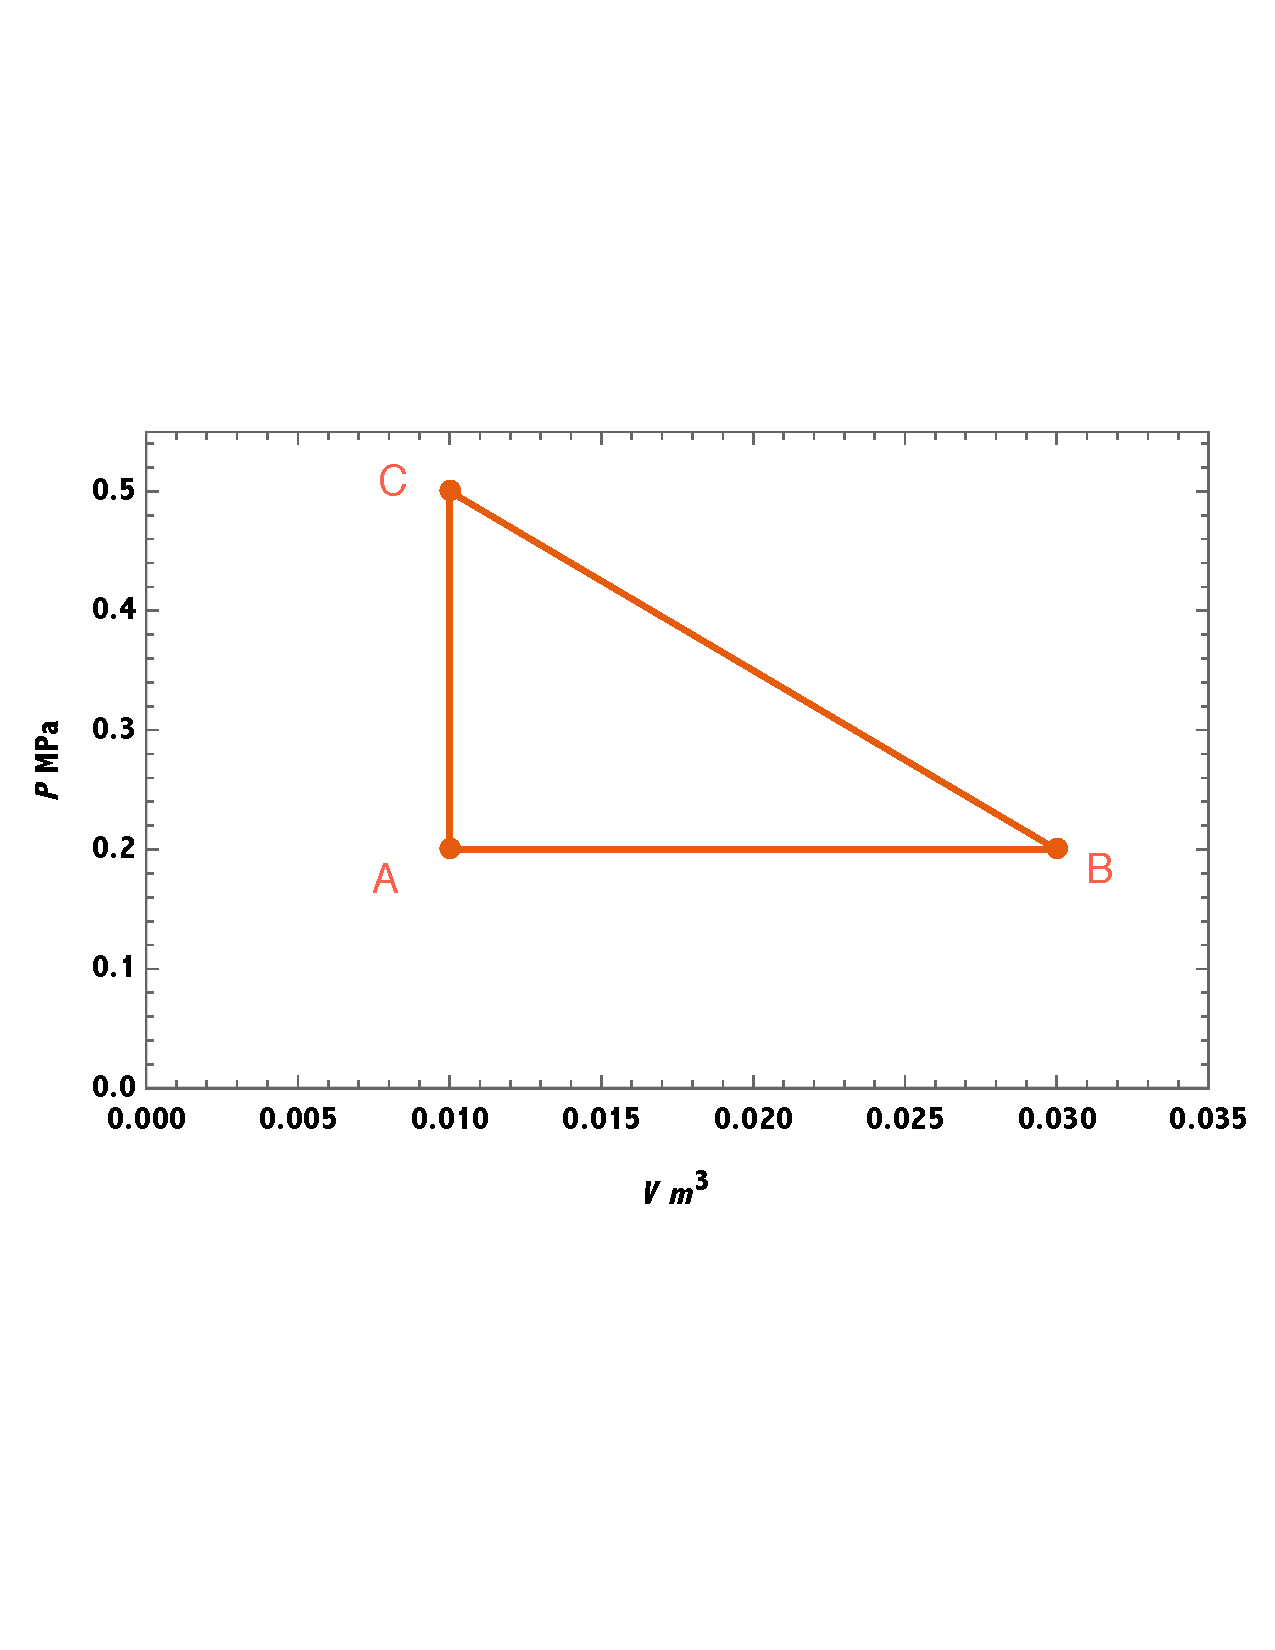
\includegraphics[width=0.6\textwidth]{./Figure1-annotated.pdf}
\end{center}
\end{center}

\begin{enumerate}
\item The system starts at state \(A\), in which \(P= \SI{0.2}{MPa}\) and \(V = \SI{0.01}{m^{3}}\). It is taken quasistatically along the path shown in the figure (\(A \rightarrow B\), \(B \rightarrow C\), \(C \rightarrow A\) ).  Calculate the heat transferred from the surroundings, \(q\), and the work done on the system, \(w\), for each step along the path.

\item Calculate \(q\) and \(w\) for a quasistatic process starting at \(A\) and ending at \(B\) along the path \(P=a + b(V-c)^{2}\), where \(a = \SI{0.1}{MPa}\), \(b= \SI{1e3}{MPa. m^{-6}}\), and \(c = \SI{0.02}{m^{3}}\).

\item The system exchanges both heat and work with its surroundings along the paths above. An \emph{adiabat} is a particular quasistatic path along which work is done but no heat is transferred.  Find the form of the adiabats \(P=P(V)\) for the system described by \(U = \frac{5}{2} PV +C\).  (\emph{Hint:} If \(\dbar q_\text{qs} = 0\), then \(dU = \dbar w_\text{qs} = -PdV\).  What else does \(dU\) equal?)
\end{enumerate}

\section{Is it fundamental enough?}
\label{sec:orgae1740c}
The following ten equations are purported to be fundamental equations for
various thermodynamic systems.  Five, however, are inconsisent with the basic
  postulates of a fundamental equation and are thus unphysical.  For each, plot
  the relationship between \(S\) and \(U\) and identify the five that are
  unacceptable. \(v_0\), \(\theta\), and \(R\) are all positive constants and, in the
  case of fractional exponents, the real positive root is to be implied.

\[ S = \left ( \frac{R^2}{v_0\theta} \right )^{1/3}\left ( NVU \right
)^{1/3}\hspace{20pt}
S = \left ( \frac{R}{\theta^2} \right )^{1/3}\left ( \frac{NU}{V} \right)^{2/3} \]

\[ S = \left ( \frac{R}{\theta} \right )^{1/2}\left ( NU + \frac{R\theta
    V^2}{v_0^2} \right)^{1/2}
\hspace{20pt}
S = \left ( \frac{R^2\theta}{v_0^3} \right ) \frac{V^3}{NU}  \]

\[ S = \left ( \frac{R^3}{v_0\theta^2} \right )^{1/5}\left ( N^2U^2V
 \right)^{1/5}
\hspace{20pt}
S = NR \ln \left ( \frac{UV}{N^2 R \theta v_0}  \right )  \]

\[ S = \left ( \frac{NRU}{\theta} \right )^{1/2}\exp
\left (-\frac{V^2}{2N^2v_0^2}
 \right )
\hspace{20pt}
S = \left ( \frac{NRU}{\theta} \right )^{1/2}\exp
\left (-\frac{UV}{NR\theta v_0} \right ) \]

\[ U = \left ( \frac{NR\theta V}{v_0} \right ) \left ( 1+\frac{S}{NR} \right ) \exp
  \left (-S/NR \right )
\hspace{20pt}
U = \left ( \frac{v_0\theta}{R} \right ) \frac{S^2}{V} \exp\left ( S/NR \right )
 \]

\section{Find your equilibrium}
\label{sec:orgc31ab60}
The fundamental equations of both systems \(A\) and \(B\) are \[ S = \left (
\frac{R^2}{v_0\theta} \right )^{1/3} \left ( N V U \right )^{1/3} \] The volume
and mole number of system \(A\) are \SI{9e-6}{m^3} and \SI{3}{\mole},
respectively, and of system \(B\) are \SI{4e-6}{m^3} and \SI{2}{\mole},
respectively.  First suppose \(A\) and \(B\) are completely isolated from one
another.  Plot the total entropy \(S_A + S_B\) as function of \(U_A/(U_A + U_B)\),
where \(U_A + U_B = 80\) J. If \(A\) and \(B\) were connected by a diathermal wall and
the pair allowed to come to equilibrium, what would \(U_A\) and \(U_B\) be?

\section{Exactly right}
\label{sec:orgd8f6b9f}
The Helmholtz energy \(A\) is a thermodynamic state function.  Show that
\[ \left (\frac{\partial A}{\partial V}\right )_T = - P \ \text{and}\ \left
  (\frac{\partial A}{\partial T}\right )_V = - S\ \text{implies}\
 \left (\frac{\partial S}{\partial V}\right )_T = \left
  (\frac{\partial P}{\partial T}\right )_V  \]

\section{A difference of degree}
\label{sec:org5232f23}
Determine whether the following five expressions are homogeneous and, if so, what
  their degree of homogeneity is:
\[ u=x^2y + xy^2 +3xyz \]
\[ u=\sqrt{x+y} \]
\[u=\frac{x^3+x^2y+y^3}{x^2+xy+y^2}\]
\[u=e^{-y/x} \]
\[u=\frac{x^2+3xy+2y^3}{y^2} \]
\end{document}